\documentclass[journal]{IEEEtran}

\usepackage[utf8]{inputenc}
\usepackage[T1]{fontenc}
\usepackage{graphicx}
\usepackage{booktabs}
\usepackage{array}
\usepackage{tabularx}
\usepackage{multirow}
\usepackage{url}
\usepackage{cite}
\usepackage{amsmath}
\usepackage{balance}
\usepackage{xcolor}
\usepackage[hidelinks]{hyperref}

\newcommand{\logminer}{Logminer}
\newcommand{\doiurl}[1]{\href{https://doi.org/#1}{\nolinkurl{doi:#1}}}

\begin{document}

\title{Adaptive Multi-Agent AI Framework for Real-Time Log Anomaly Detection in Distributed Systems}

\author{Andr\'e Olivier Marhegane Bitati,
G\'ed\'eon Nkishi Djenga,
Jean-Pierre Mugisha Muhire,
Josu\'e Lungi Selemani,
Christian Kutabuna Kubakisa,
Jeff Mugaruka Chihyoka,
and Kyandoghere Kyamakya%
\thanks{Andr\'e Olivier Marhegane Bitati, G\'ed\'eon Nkishi Djenga, Jean-Pierre Mugisha Muhire, Josu\'e Lungi Selemani, Christian Kutabuna Kubakisa and Jeff Mugaruka Chihyoka are with the Faculty of Engineering (Polytechnic), Department of Electrical and Computer Engineering, University of Kinshasa, Kinshasa, DR Congo.}%
\thanks{Kyandoghere Kyamakya is with the Institute for Smart Systems Technologies, University of Klagenfurt, Klagenfurt, Austria.}%
\thanks{Corresponding author: Andr\'e Olivier Marhegane Bitati. Emails: aolivier.marhegane@unikin.ac.cd, gedeon.nkishi@unikin.ac.cd, tomsmugisha@unikin.ac.cd, josue.lungi@unikin.ac.cd, christian.kutabuna@unikin.ac.cd, Mugarukachihyoka@gmail.com, kyandoghere.kyamakya@aau.at.}}

\maketitle

\begin{abstract}
This article presents an extended experimental evaluation of \logminer, a lightweight multi-agent framework for real-time anomaly detection in heterogeneous system, network and distributed-system logs. The system decomposes the workflow into specialized software agents for collection, parsing, normalization, family-aware routing, anomaly detection, correlation, dashboard exploration and audit. In accordance with the second article trajectory defined in the project plan, the focus is distributed architecture, resilience, scalability-oriented evaluation and operational behavior under heterogeneous data, robustness constraints, local quasi-real-time execution and resource monitoring.

The evaluation covers Windows logs, Wazuh exports, Linux/auth logs, HDFS, BGL, CICIDS2017 and UNSW/CIC-DDoS data. Supervised Random Forest models reach F1-scores of 0.916602 on Linux/auth, 0.997163 on CICIDS2017 and 0.999965 on UNSW/CIC-DDoS. Wazuh exports contain 122,563 events and produce 3,676 non-supervised anomaly candidates. A quasi-real-time benchmark reports a mean workflow latency of 10.6473 seconds over five cycles of 8,537 lines, while a 30-cycle resource campaign reports a mean workflow duration of 9.3300 seconds. A new local parallel campaign, using three detector workers on 500 labeled events per cycle, completes five cycles with a mean duration of 3.6232 seconds, a mean maximum machine CPU load of 17.1725\% and a mean maximum RAM footprint of 176.89 MB. The discussion explicitly addresses false positives, HDFS limitations, synchronous buffering, bounded supervisor policies, local parallel execution and the difference between anomaly candidates and confirmed attacks.
\end{abstract}

\begin{IEEEkeywords}
log anomaly detection, multi-agent system, lightweight machine learning, cybersecurity monitoring, resource analysis, robustness, Wazuh, SIEM complement
\end{IEEEkeywords}

\section{Introduction}
Security monitoring pipelines increasingly face heterogeneous, noisy and high-volume logs. Operating systems, SIEM/HIDS exports, cloud audit records, distributed-system traces and network-flow datasets expose different fields, temporal structures and anomaly semantics. This makes a single monolithic detector difficult to deploy and difficult to interpret.

\logminer{} is a lightweight prototype designed around specialized software agents rather than a single opaque processing block. The first article focused on the family-aware routing architecture. Following the project plan for the second IEEE Access article, this manuscript extends the evaluation toward distributed architecture, resilience, scalability, robustness, resource behavior, quasi-real-time execution and operational positioning. The term agent is used in an architectural sense: agents are software modules with bounded responsibilities, explicit message exchange and workflow coordination. The prototype does not claim cognitive autonomy, reinforcement-learning control or FIPA-style negotiation.

The contributions of this article are:
\begin{enumerate}
    \item an extended evaluation of lightweight supervised and non-supervised models across heterogeneous log families;
    \item a robustness and resilience analysis covering unknown, incomplete and multi-format logs;
    \item a quasi-real-time, 30-cycle resource and local parallel-execution evaluation of the workflow;
    \item an operational discussion of buffering, back-pressure, supervisor stability, false positives and complementarity with standard tools such as Wazuh, OSSEC and fail2ban.
\end{enumerate}

The paper uses cautious claims. Non-supervised detections are treated as anomaly candidates. The current distribution is local and service-oriented, not yet a full multi-machine SOC deployment. HDFS/BGL-style sequential logs are identified as requiring template-based and temporal extensions.

\section{System Overview}
\subsection{Multi-Agent Workflow}
Fig.~\ref{fig:architecture} summarizes the current \logminer{} workflow. The collector retrieves local or exported logs; the parser extracts structure; the normalizer maps records to a common event contract; the router selects a compatible family branch; the detector produces anomaly candidates; the correlator groups candidates into incidents; and the dashboard/audit layer supports analyst validation.

\begin{figure}[t]
    \centering
    
\includegraphics[width=\linewidth]{figures/fig_architecture_logminer.pdf}
    \caption{Logical architecture of \logminer. Heterogeneous logs are collected, parsed, normalized, routed to compatible detector branches and correlated into analyst-readable incident candidates.}
    \label{fig:architecture}
\end{figure}

The implementation uses Python, scikit-learn models, local file artifacts, JSONL bus traces and FastAPI endpoints. Redis Streams is now available as an optional queued-execution layer: FastAPI can enqueue workflows into a persistent job stream, and external workers can consume them through Redis consumer groups. MQTT is also available as an optional pub/sub channel for lightweight collectors and real-time notifications. This article is therefore the appropriate venue for operational discussion of Redis/MQTT behavior, worker execution, pending jobs, resilience and the remaining back-pressure limits; durable SOC-scale asynchronous scaling still requires longer stress campaigns and production policies.

\subsection{Model Portfolio}
The model portfolio combines supervised Random Forest models for labeled tabular families and non-supervised Isolation Forest or ensemble-style detectors for unlabeled or partially labeled sources. Fig.~\ref{fig:portfolio} shows the family-aware model portfolio.

\begin{figure}[t]
    \centering
    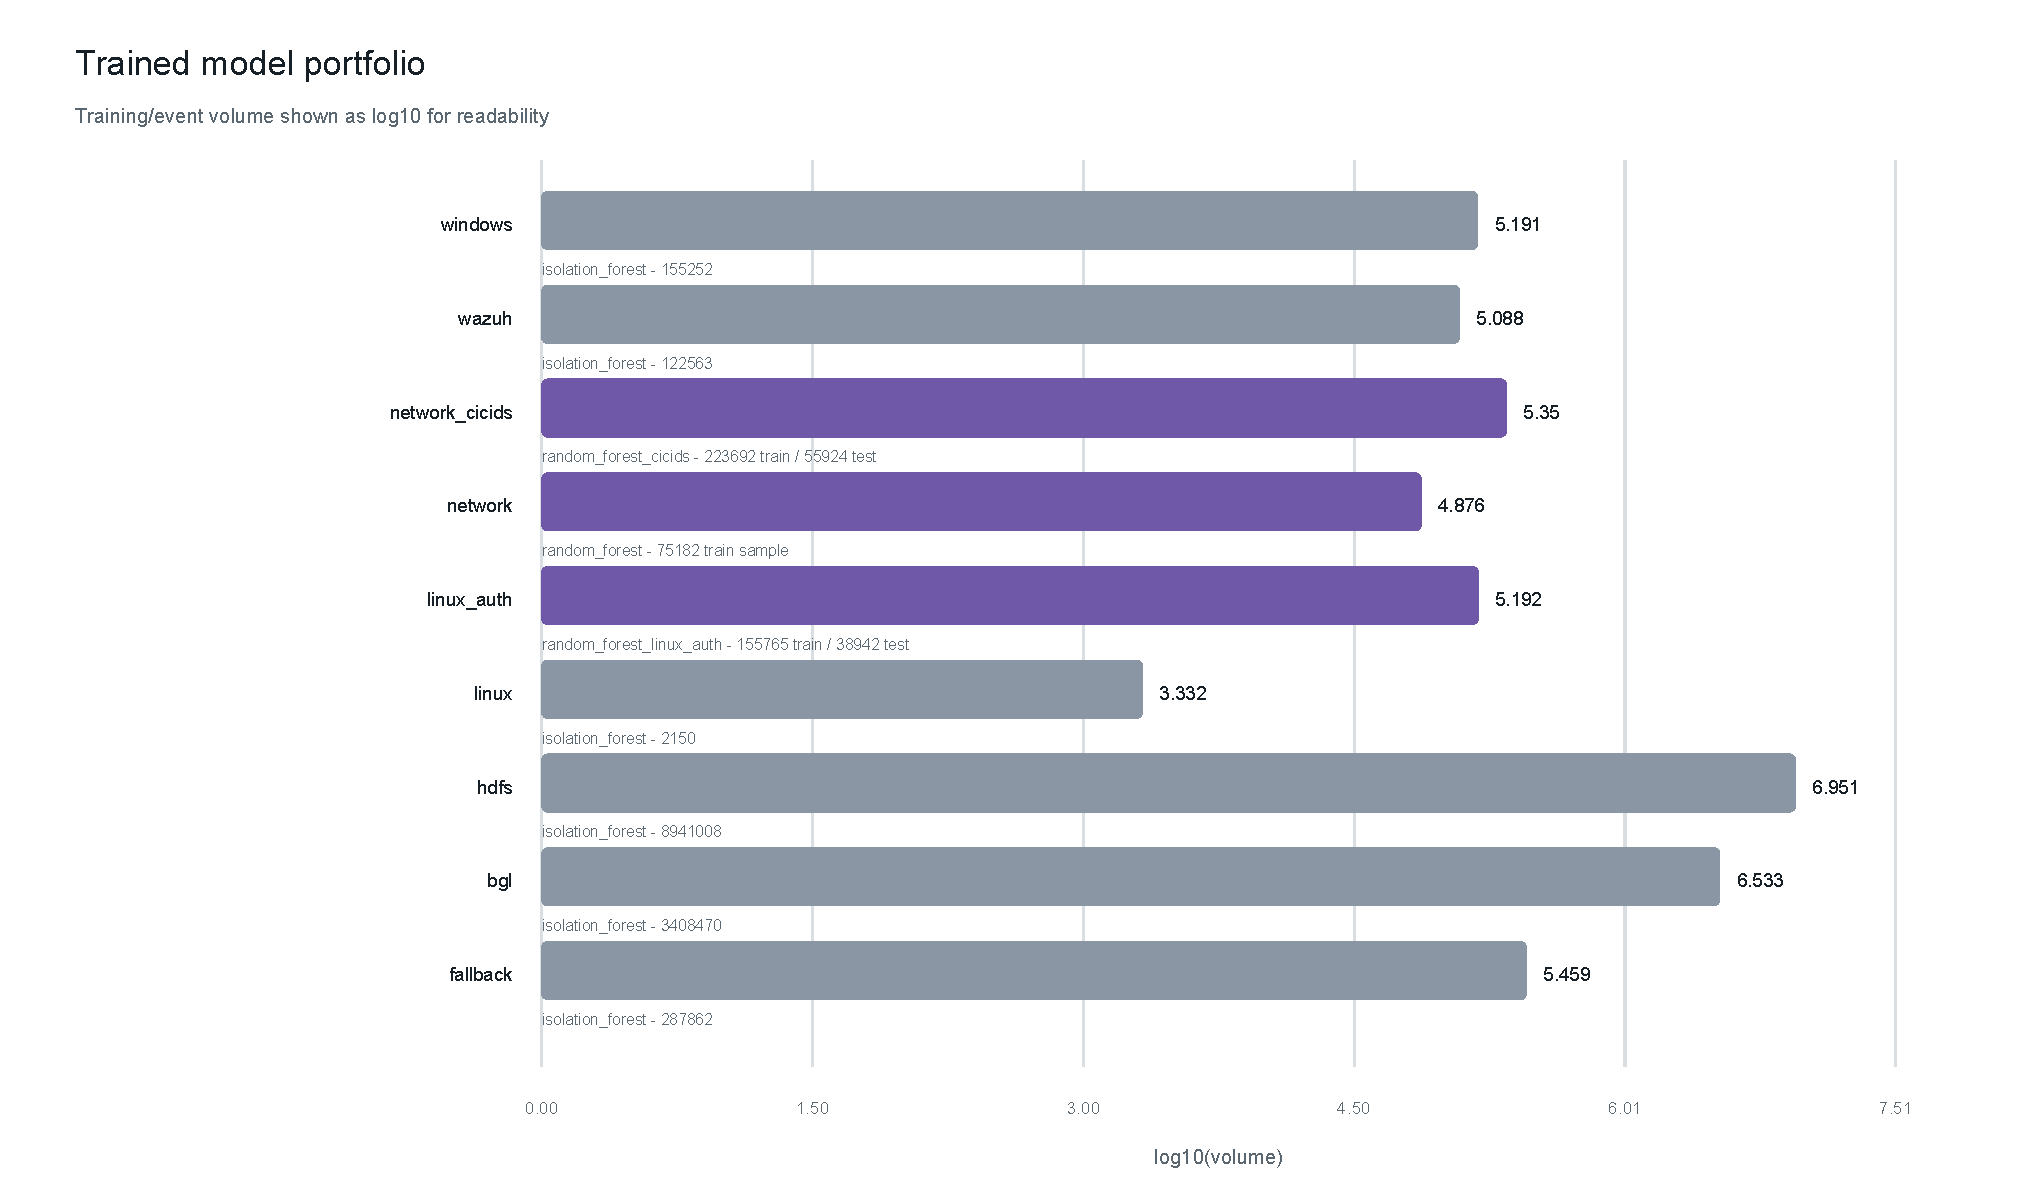
\includegraphics[width=\linewidth]{figures/fig_model_portfolio_scale.pdf}
    \caption{Model portfolio used by \logminer{} across Windows, Wazuh, Linux/auth, network, HDFS, BGL and fallback families.}
    \label{fig:portfolio}
\end{figure}

\section{Evaluation Methodology}
\subsection{Datasets and Scenarios}
Table~\ref{tab:datasets} lists the evaluation families. The protocol combines local logs, SIEM/HIDS exports, public system logs, public network-flow datasets and robustness cases.

\begin{table*}[t]
\caption{Datasets and scenarios used in the extended evaluation}
\label{tab:datasets}
\centering
\scriptsize
\begin{tabularx}{\textwidth}{p{2.3cm}p{3.2cm}p{3.0cm}X}
\toprule
\textbf{Category} & \textbf{Source} & \textbf{Nature} & \textbf{Objective} \\
\midrule
Local real & Windows Event/Application/System/Security & Windows system logs & Test local collection, parsing and non-supervised candidate detection \\
Real/SIEM & Wazuh exports & SIEM/HIDS alerts and events & Evaluate non-supervised anomaly candidates and overlap with Wazuh grouping \\
Real tabular & Linux/auth & Labeled authentication logs & Supervised model evaluation and false positive analysis \\
Public system & HDFS & Distributed-system logs with labels & Evaluate limits of row-level features on sequential logs \\
Public system & BGL & BlueGene/L logs with labels & Evaluate lightweight models on HPC logs \\
Public network & CICIDS2017 & Labeled network flows & Supervised detection of attack classes \\
Public network & UNSW/CIC-DDoS & Network/DDoS flows & Chunk-based supervised evaluation \\
Robustness & Apache, CEF/LEEF, CloudTrail, Linux auth, incomplete log & Multi-format and corrupted input & Test conservative preservation of unknown records \\
\bottomrule
\end{tabularx}
\end{table*}

\subsection{Metrics and Reproducibility}
For labeled datasets, the evaluation reports F1-score and false positive rates. For unlabeled operational exports, the output is explicitly interpreted as anomaly candidates. Workflow latency, CPU and memory consumption are evaluated separately because they characterize deployment feasibility rather than detection quality.

The routing strategy uses fixed, interpretable policy parameters. Large differences between routing constants are treated as rule-specific evidence, not as globally calibrated learned coefficients. Heavy constants are attached to discriminative markers or fallback-only cases, and the router combines scores with mandatory evidence checks. Softmax or MinMax score normalization is left for future calibration because it may inflate weak evidence when all families are poorly supported.

\section{Experimental Results}
\subsection{Detection Results}
Table~\ref{tab:main_results} summarizes the main detection results. The strongest supervised results are obtained on Linux/auth, CICIDS2017 and UNSW/CIC-DDoS. HDFS remains weak with lightweight row-level features, which confirms that sequential distributed-system logs require semantic parsing and temporal modeling.

\begin{table}[t]
\caption{Principal detection results}
\label{tab:main_results}
\centering
\scriptsize
\begin{tabularx}{\linewidth}{p{1.6cm}p{1.8cm}X}
\toprule
\textbf{Family} & \textbf{Model} & \textbf{Main result} \\
\midrule
Linux/auth & Random Forest & F1 = 0.916602 \\
CICIDS2017 & Random Forest & F1 = 0.997163 \\
UNSW/CIC-DDoS & Random Forest & F1 = 0.999965 \\
Wazuh & Isolation Forest & 122,563 events; 3,676 anomaly candidates \\
BGL & Ensemble & Best selection around F1 = 0.994333 \\
HDFS & Ensemble & Best selection around F1 = 0.599333 \\
\bottomrule
\end{tabularx}
\end{table}

\begin{figure}[t]
    \centering
    
\includegraphics[width=\linewidth]{figures/fig_supervised_models_f1.pdf}
    \caption{F1-score of supervised Random Forest models on Linux/auth, CICIDS2017 and UNSW/CIC-DDoS families.}
    \label{fig:supervised}
\end{figure}

\begin{figure}[t]
    \centering
    
\includegraphics[width=\linewidth]{figures/fig_validation_selection_f1.pdf}
    \caption{Validation-based model selection across log families. HDFS remains difficult for lightweight row-level representations.}
    \label{fig:validation}
\end{figure}

\subsection{False Positives and HDFS Limitation}
False positives directly affect analyst workload. Table~\ref{tab:falsepos} reports representative false positive rates. HDFS reaches 200.333 false positives per 1000 lines, which is a structural limitation of the current line-level representation rather than a failure of the routing architecture itself.

\begin{table}[t]
\caption{Representative false positive results}
\label{tab:falsepos}
\centering
\scriptsize
\begin{tabular}{l r r}
\toprule
\textbf{Dataset} & \textbf{FPR} & \textbf{FP/1000} \\
\midrule
Linux/auth & 0.047250 & 29.120 \\
CICIDS2017 & 0.001933 & 1.037 \\
UNSW/CIC-DDoS & 0.001709 & 0.001 \\
BGL & 0.005667 & 2.833 \\
HDFS & 0.400667 & 200.333 \\
Simulated Windows & 0.000000 & 0.000 \\
\bottomrule
\end{tabular}
\end{table}

\begin{figure}[t]
    \centering
    
\includegraphics[width=\linewidth]{figures/fig_false_positive_rates.pdf}
    \caption{False positive rates observed by log family and model. HDFS highlights the limitation of lightweight row-level features for sequence-oriented logs.}
    \label{fig:falsepos}
\end{figure}

For HDFS/BGL-like sources, the modular event contract can route logs to a Drain-like semantic parsing agent followed by sequence-aware detection, while preserving lighter tabular branches for Linux/auth and network-flow families.

\subsection{Family-Aware Ablation}
Fig.~\ref{fig:ablation} summarizes the controlled common-space ablation. This result is deliberately conservative: routing alone does not guarantee universal F1 improvement when all families are forced into the same minimal representation. The operational value of routing is that it enables compatible native feature spaces and specialized detector branches.

\begin{figure}[t]
    \centering
    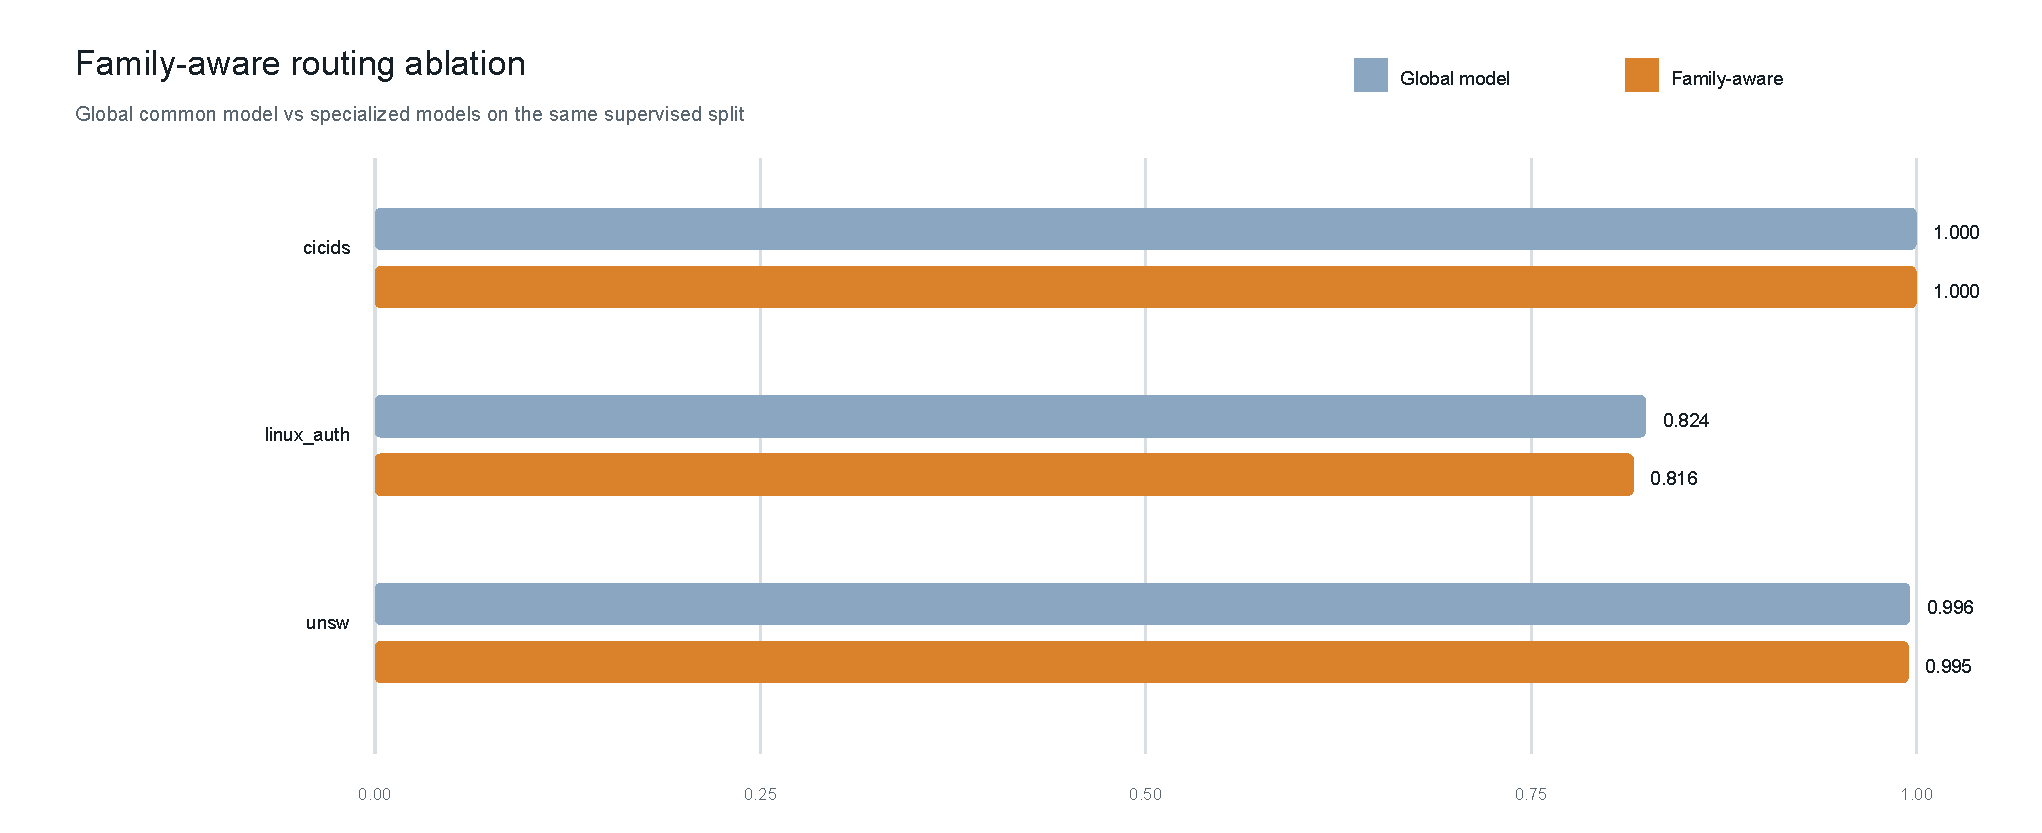
\includegraphics[width=\linewidth]{figures/fig_family_routing_ablation.pdf}
    \caption{Controlled common-space ablation. The family-aware strategy should be read as controlled specialization, not as a universal F1 improvement claim.}
    \label{fig:ablation}
\end{figure}

\subsection{Robustness}
The robustness scenario covers Apache, CEF/LEEF, CloudTrail, Linux auth and an incomplete log. Unknown or corrupted records are preserved as unknown records instead of breaking the workflow.

\begin{figure}[t]
    \centering
    
\includegraphics[width=\linewidth]{figures/fig_robustness_multiformat.pdf}
    \caption{Robustness check on multi-format inputs. Unknown or incomplete entries are preserved instead of silently lost.}
    \label{fig:robustness}
\end{figure}

\section{Resource and Workflow Analysis}
\subsection{Quasi-Real-Time Benchmark}
The FastAPI workflow was evaluated over five cycles of 8,537 lines per cycle. The mean workflow latency is 10.6473 seconds, with a minimum of 3.0865 seconds and a maximum of 19.8163 seconds.

\begin{table}[t]
\caption{Quasi-real-time workflow benchmark}
\label{tab:realtime}
\centering
\scriptsize
\begin{tabular}{l r}
\toprule
\textbf{Indicator} & \textbf{Value} \\
\midrule
Completed cycles & 5/5 \\
Lines per cycle & 8,537 \\
Minimum latency & 3.0865 s \\
Mean latency & 10.6473 s \\
Maximum latency & 19.8163 s \\
\bottomrule
\end{tabular}
\end{table}

\begin{figure}[t]
    \centering
    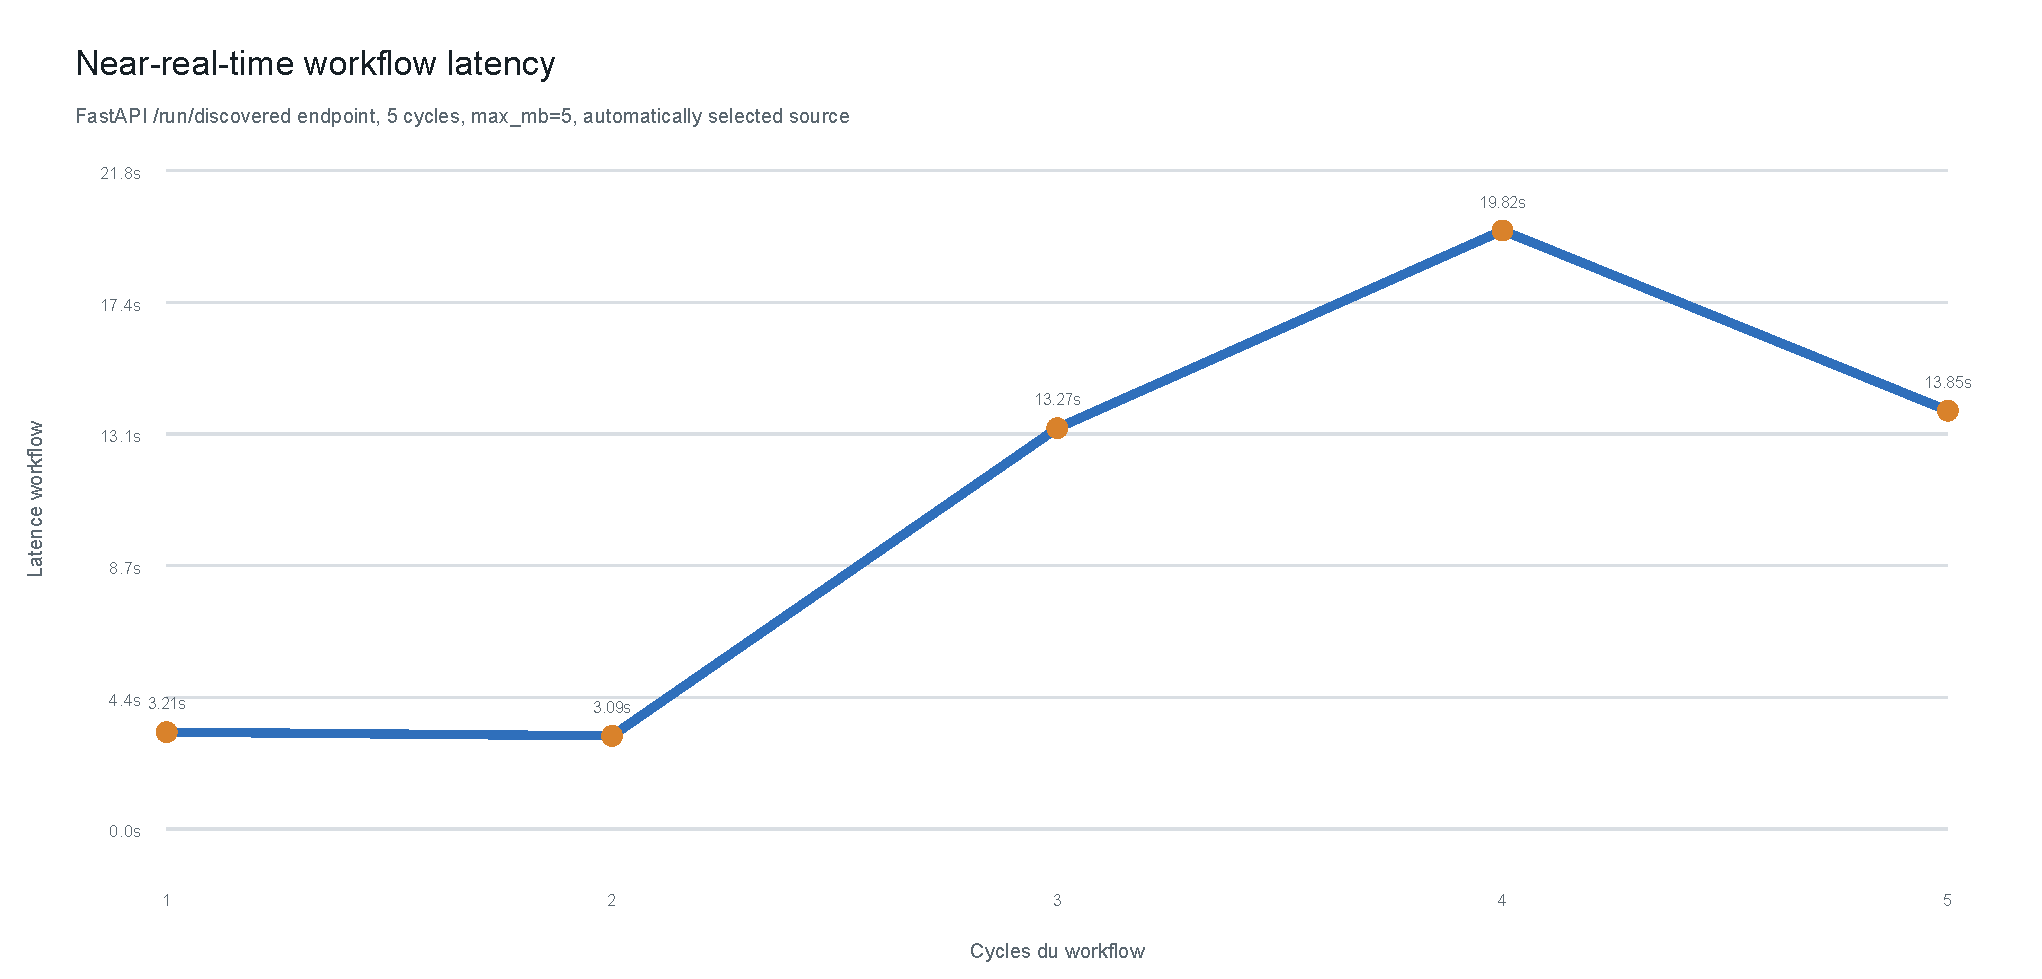
\includegraphics[width=\linewidth]{figures/fig_realtime_workflow_latency.pdf}
    \caption{Workflow latency observed during the quasi-real-time FastAPI benchmark.}
    \label{fig:latency}
\end{figure}

\subsection{Thirty-Cycle Resource Campaign}
The 30-cycle resource campaign reports a mean workflow duration of 9.3300 seconds and a maximum duration of 21.6007 seconds. The API/orchestrator process averages 187.82 MB RAM, while the Logminer process averages 495.41 MB and reaches 655.39 MB.

\begin{table}[t]
\caption{Thirty-cycle resource campaign}
\label{tab:resources}
\centering
\scriptsize
\begin{tabular}{l r}
\toprule
\textbf{Indicator} & \textbf{Value} \\
\midrule
Completed cycles & 30/30 \\
Lines per cycle & 8,537 \\
Mean workflow duration & 9.3300 s \\
Maximum workflow duration & 21.6007 s \\
API/orchestrator mean RAM & 187.82 MB \\
Logminer mean RAM & 495.41 MB \\
Logminer maximum RAM & 655.39 MB \\
\bottomrule
\end{tabular}
\end{table}

\begin{figure}[t]
    \centering
    
\includegraphics[width=\linewidth]{figures/fig_resource_campaign_multicycle.pdf}
    \caption{CPU/RAM behavior observed during the 30-cycle campaign. The measurements support local feasibility but not industrial SOC throughput.}
    \label{fig:resources}
\end{figure}

\subsection{Local Parallel Execution Campaign}
The implementation now exposes parallelism at several levels: independent detector comparison tasks, parser execution over multiple files, chunk-based supervised inference, grouped correlation and parallel supervisor campaigns with isolated per-cycle memory files. To separate this mode from the previous synchronous resource campaign, a dedicated local experiment executed \texttt{model\_compare} with three detector workers on a synthetic labeled CSV of 500 events. Five cycles completed successfully. The mean workflow duration was 3.6232 seconds, with a maximum of 6.0172 seconds. The mean maximum machine CPU load was 17.1725\%, and the mean maximum RAM footprint was 176.89 MB.

\begin{table}[t]
\caption{Local parallel resource campaign}
\label{tab:parallel_resources}
\centering
\scriptsize
\begin{tabular}{l r}
\toprule
\textbf{Indicator} & \textbf{Value} \\
\midrule
Completed cycles & 5/5 \\
Events per cycle & 500 \\
Parallel detector workers & 3 \\
Mean workflow duration & 3.6232 s \\
Maximum workflow duration & 6.0172 s \\
Mean maximum machine CPU & 17.1725\% \\
Mean maximum RAM & 176.89 MB \\
\bottomrule
\end{tabular}
\end{table}

\begin{figure}[t]
    \centering
    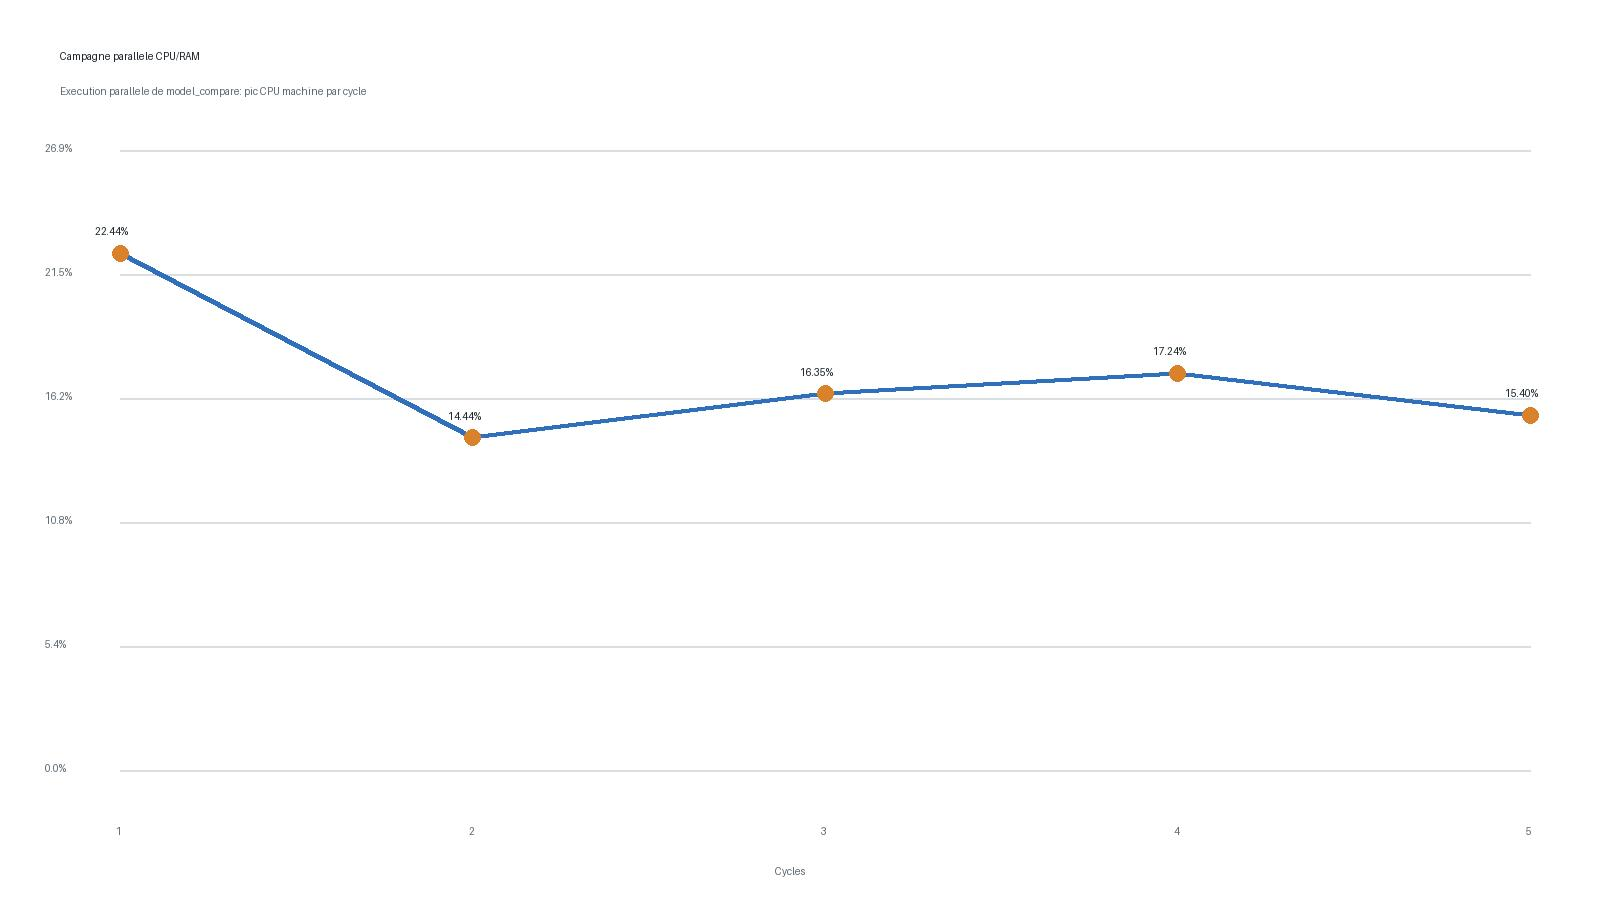
\includegraphics[width=\linewidth]{figures/fig_parallel_resource_campaign.pdf}
    \caption{CPU peaks observed during the local parallel detector campaign. The experiment validates local multi-worker execution, while broader queue throughput and multi-machine back-pressure remain future work.}
    \label{fig:parallel_resources}
\end{figure}

\subsection{Buffering and Back-Pressure}
The current buffering strategy is local and conservative. Collectors and parsers persist raw files, manifests, normalized records and JSONL bus messages before detection. The detector processes bounded samples or prepared batches rather than an unbounded memory queue. If detection lags behind collection, the backlog remains visible in files and traces, but the prototype does not yet implement production-grade admission control, retry policies, priority scheduling or durable back-pressure. A Kafka, MQTT, Redis Streams or equivalent broker is required for sustained asynchronous SOC ingestion.

\section{Supervisor Stability and Stress Behavior}
The SupervisorAgent performs bounded policy-based workflow control. It observes sources and resources, selects a source, adjusts sample size and correlation window, launches workflow steps and records decisions. A 30-cycle campaign showed stable completion, but this is a functional stability check, not proof of long-term autonomy.

The current policies cap correlation windows at 20 minutes for repeated fallback routes and 30 minutes for sequential HDFS/BGL-style sources. Sampling is reduced to a lower bounded profile rather than repeatedly divided. Under prolonged stress, such as a multi-hour stream of corrupted logs, this behavior protects resources but may create an observability blind spot if fallback routing and minimal sampling become persistent. Therefore, prolonged fallback should trigger fallback-rate alerts, degradation budgets, source quarantine and analyst notification in a future production version.

\section{Wazuh and Standard Tool Complementarity}
The Wazuh export contains 122,563 events and 3,676 \logminer{} anomaly candidates. Fig.~\ref{fig:wazuh} illustrates overlap between Wazuh event groups and \logminer{} candidates. This comparison should not be interpreted as replacement. Wazuh provides mature HIDS/SIEM rules, decoders and operational workflows; \logminer{} adds a lightweight analytical layer for anomaly candidates, model specialization and correlation.

\begin{figure}[t]
    \centering
    
\includegraphics[width=\linewidth]{figures/fig_wazuh_logminer_overlap.pdf}
    \caption{Overlap between Wazuh event groups and \logminer{} anomaly candidates. The objective is complementarity, not replacement.}
    \label{fig:wazuh}
\end{figure}

\section{Threats to Validity}
Internal validity is limited because datasets, feature spaces and model families differ. The ablation mitigates this risk but also shows that family-aware routing is not universally superior under a common minimal representation. External validity is limited by local execution and selected datasets. Operational validity is limited because non-supervised outputs require analyst validation, correlation quality is not yet measured against analyst-labeled incidents and the current workflow is only partially parallelized. HDFS results show that sequence-oriented logs need Drain-like templates and temporal detectors. The sequential and parallel resource campaigns support local feasibility, not production SOC throughput.

\section{Conclusion}
This article prepared an extended evaluation-oriented view of \logminer. Results show strong supervised performance on Linux/auth, CICIDS2017 and UNSW/CIC-DDoS, useful Wazuh anomaly-candidate generation, robust preservation of unknown records and feasible local quasi-real-time operation. The added parallel campaign shows that independent detector execution can be exploited locally with measurable CPU/RAM behavior. The main limitations are also explicit: high HDFS false positives, partial synchronous buffering, local-only resource measurements, bounded but non-learning supervisor control and the need for durable asynchronous scaling. Future work includes semantic parsing for sequential logs, calibrated routing confidence, distributed message buses, active analyst feedback, automatic degradation watchdogs and integration with mature SIEM/HIDS platforms.

\section*{Declaration of Generative AI and AI-Assisted Technologies}
The authors used AI-assisted writing tools to improve language clarity, structure and readability during manuscript preparation. The authors reviewed, edited and validated the technical content and take full responsibility for the final manuscript.

\balance
\begin{thebibliography}{00}
\bibitem{denning1987intrusion} D. E. Denning, ``An intrusion-detection model,'' \emph{IEEE Transactions on Software Engineering}, vol. SE-13, no. 2, pp. 222--232, 1987, \doiurl{10.1109/TSE.1987.232894}. Available: \url{https://www.cs.colostate.edu/~cs656/reading/ieee-se-13-2.pdf}.
\bibitem{axelsson2000intrusion} S. Axelsson, ``Intrusion detection systems: A survey and taxonomy,'' Technical Report, Chalmers University of Technology, 2000. Available: \url{https://www.cse.msu.edu/~cse960/Papers/security/axelsson00intrusion.pdf}.
\bibitem{sommer2010outside} R. Sommer and V. Paxson, ``Outside the closed world: On using machine learning for network intrusion detection,'' in \emph{IEEE Symposium on Security and Privacy}, 2010, pp. 305--316, \doiurl{10.1109/SP.2010.25}.
\bibitem{chandola2009anomaly} V. Chandola, A. Banerjee, and V. Kumar, ``Anomaly detection: A survey,'' \emph{ACM Computing Surveys}, vol. 41, no. 3, pp. 1--58, 2009, \doiurl{10.1145/1541880.1541882}.
\bibitem{buczak2016survey} A. L. Buczak and E. Guven, ``A survey of data mining and machine learning methods for cyber security intrusion detection,'' \emph{IEEE Communications Surveys and Tutorials}, vol. 18, no. 2, pp. 1153--1176, 2016, \doiurl{10.1109/COMST.2015.2494502}.
\bibitem{khraisat2019survey} A. Khraisat, I. Gondal, P. Vamplew, and J. Kamruzzaman, ``Survey of intrusion detection systems: Techniques, datasets and challenges,'' \emph{Cybersecurity}, vol. 2, no. 20, 2019, \doiurl{10.1186/s42400-019-0038-7}.
\bibitem{he2016drain} P. He, J. Zhu, Z. Zheng, and M. R. Lyu, ``Drain: An online log parsing approach with fixed depth tree,'' in \emph{IEEE International Conference on Web Services}, 2017, pp. 33--40, \doiurl{10.1109/ICWS.2017.13}. Available: \url{https://jiemingzhu.github.io/pub/pjhe_icws2017.pdf}.
\bibitem{du2017deeplog} M. Du, F. Li, G. Zheng, and V. Srikumar, ``DeepLog: Anomaly detection and diagnosis from system logs through deep learning,'' in \emph{ACM CCS}, 2017, pp. 1285--1298, \doiurl{10.1145/3133956.3134015}.
\bibitem{balasubramaniyan1998aafid} J. S. Balasubramaniyan, J. O. Garcia-Fernandez, D. Isacoff, E. Spafford, and D. Zamboni, ``An architecture for intrusion detection using autonomous agents,'' in \emph{Annual Computer Security Applications Conference}, 1998, pp. 13--24. Available: \url{https://zzamboni.org/files/pubs/aafid-acsac98.pdf}.
\bibitem{nist80092} National Institute of Standards and Technology, ``Guide to computer security log management,'' NIST Special Publication 800-92, 2006, \doiurl{10.6028/NIST.SP.800-92}.
\bibitem{rfc5424} R. Gerhards, ``The Syslog Protocol,'' RFC 5424, 2009, \doiurl{10.17487/RFC5424}.
\end{thebibliography}

\end{document}
